\chapter{Estimation of Bernstein-Sato zero-loci}\label{ch: ChapterRelHol}
Let $F = (f_1,\ldots,f_r)\in \C^n\to \C^r$ be a tuple of polynomials.
Introduce new variables $s = (s_1,\ldots, s_r)$ and fix a tuple of natural numbers $a = (a_1,\ldots, a_r) \in \mathbb{Z}_{\geq a}^r$ such that the product $f_1^{a_1}\ldots f_r^{a_r}$ is not invertible.
The monovariate Bernstein-Sato polynomial in \cref{sec: MonodromyBS} is generalised by the Bernstein-Sato ideal $B_F^{a}$ which consists of all polynomials $b(s)\in \C[s]$ such that
$$b(s) F^s \in \D_{\C^n}[s]F^{s+a}$$
where $F^s = f_1^{s_1}\cdots f_r^{s_r}$.
The main purpose of this chapter is to generalise the estimate by Lichtin and Kashiwara given in \cref{sec: sec: MonodromyBS} to the zero locus of $B_F^a$.

\Cref{sec: BSIdeal} provides an introduction to Bernstein-Sato zero loci and the available results on their estimation.
It turns out that the $\D_X$-modules encoding the Bernstein-Sato relations are no longer holonomic due to the new variables $s_i$.
This is essentially the problem which has been surmounted in \cite{budur2020zeroI} and \cite{budur2020zeroII} in order to prove a topological interpretation of $Z(B_F^a)$.
We adapt the technique from these papers to suit our goal.
The corresponding notions are introduced in \cref{sec: DXS}.
The proof for the generalisation of Lichtin's estimate is given in \cref{sec: UpperBound}.
This establishes an upper bound on the Bernstein-Sato zero locus.
A number of lower bounds on the Bernstein-Sato zero locus in terms of jumping walls of mixed multiplier ideals are given in \cref{sec: LowerBound}.
\section{Bernstein-Sato ideal}
Let $X$ be a smooth affine complex variety and consider a morphism $F:X\to \C^r$.
As in \Cref{ex: fs} let $\D_X[s]F^{s+a}$ be the $\sD_X[s]$-submodule of the free $\bC[x,f^{-1},s]$-module $\bC[x,f^{-1},s]F^{s+a}$ obtained by applying formally the operators in $\sD_X[s]$ to the symbol $F^{s+a}$ by using the usual derivation rules, where $f=f_1\ldots f_r$.
\begin{definition}
  The Bernstein-Sato zero locus associated to $F$ and $a\in \mathbb{Z}_{\geq 0}^r$ is the collection of polynomials $b(s)\in \C[s]$ such that
  $$b(s)F^s \in  \D_X[s]F^{s+a}.$$
\end{definition}
When $r>1$ the ring $\C[s]$ is not a principal ideal domain so $B_F^{a}$ may not be principal.
The zero locus of the ideal $B_F^a$ is denoted $$Z(B_F^a)\subseteq \C^r.$$
This construction extends easily to the case when $F:(X,x)\to (\bC^r,0)$ is the germ of a holomorphic map of complex manifolds.
These give rise to the so-called local Bernstein-Sato ideals $B_{F,x}^a$.
The global Bernstein-Sato ideal is known to be equal the intersection of all local $B_{F,x}^a$ for $x$ in the zero locus of $f$ \cite{brianccon2002remarques}.
\begin{example}
  Consider the case where $X=\C^2$ with $f_1 = x^{l_1}y^{k_1}$ and $f_2 = x^{l_2}y^{k_2}$.
  Then a Bernstein-Sato relation for $a = (1,1)$ may be found by acting with $\partial_x^{l_1 + l_2}\partial_y^{k_1 + k_2}$ on $F^{s+1}$.
  This shows that
  $$\prod_{i=1}^{l_1 + l_2}(l_1 s_1 + l_2 s_2 + i) \prod_{j=1}^{k_1 + k_2}  (k_1s_1 + k_2 s_2 + k) \in B_F^{1}.$$
  In this case it is straightforward to see that $B_F^{1}$ is actually the principal ideal generated by this element.
  Correspondingly, the Bernstein-Sato zero locus $Z(B_F^1)$ consists of a number of lines.
  Some lines coming from the $x$-part and others coming from the $y$-part.
  \begin{figure}[h!]
    \centering
    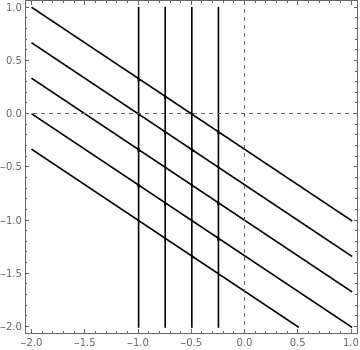
\includegraphics[width =4cm ]{Figures/MonomialBS2}
    \caption{An example of the Bernstein-Sato zero-locus $Z(B_F^1)$ in the monomial case when $F = (x^2y^4, x^3)$. The dotted lines correspond the the axes.}
  \end{figure}
  \end{example}
    In the case where $a =(1,\ldots,1)$ the Bernstein-Sato ideal $B_F^a$ can be computed using SINGULAR.
    This software package has been used to compute the examples in \cref{fig: TwoCusps} and \cref{fig: TwoCones} which were visualised using Mathematica.
    A-priori the Bernstein-Sato zero locus could have been an arbitrary affine variety, however in these examples it always seems to consist of a number of hyperplanes.
    This may be explained by the following theorem.
    \begin{theorem} \label{thrmMoreA}  (\cite[Theorem 1.1.1]{budur2020zeroII}) Let $F=(f_1,\ldots,f_r):X\ra\bC^r$ be a morphism of smooth complex affine irreducible algebraic varieties, or the germ at $x\in X$ of a holomorphic map on a complex manifold.  Let $a\in\mathbb{Z}_{\geq 0}^r$ such that $\prod_{j=1}^rf_j^{a_j}$ is not invertible. Then:
    \begin{enumerate}
    \item Every irreducible component of $Z(B_F^{a})$ of codimension 1 is a  hyperplane of type $l_1s_1+\ldots+l_rs_r+b=0$ with $l_j\in\bQ_{\ge 0}$, $b\in\bQ_{>0}$, and for each such hyperplane there exists $j$ with $a_j\ne 0$ such that $l_j>0$.
    \item Every irreducible component of  $Z(B_F^{a})$ of codimension $>1$  can be translated by an element of $\bZ^r$ inside a component of codimension 1.
    \end{enumerate}
    \end{theorem}
    For $r=1$ this is equivalent to the classical result that the roots of the Bernstein-Sato polynomial $b_f$ are negative rational numbers, due to \cite{kashiwara1976b}.
    The first part without the strict positivity of $l_j$ is due to \cite{sabbah1987proximite} and  \cite{gyoja1993bernstein}.
    The second part for the case $a=(1,\ldots,1)$ is due to \cite{maisonobe2016filtration}, a completely different proof of which was given recently by \cite{robin}.
    \begin{figure}
      \centering
      \begin{subfigure}{0.45\textwidth}
        \centering
        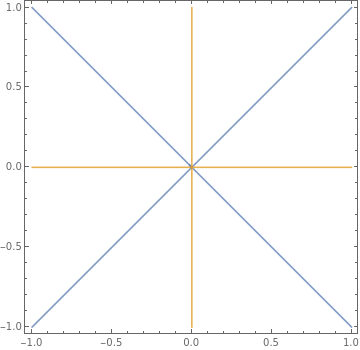
\includegraphics[width  = 4cm]{Figures/Hyperplane}
      \end{subfigure}
      \begin{subfigure}{0.45\textwidth}
        \centering
          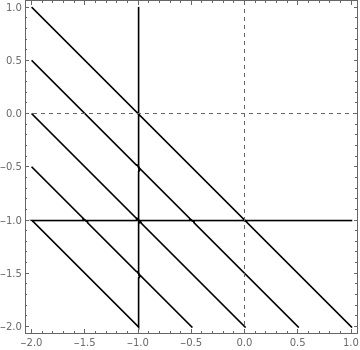
\includegraphics[width = 4cm]{Figures/HyperplaneBS}
      \end{subfigure}
      \caption{On the left: the zero loci determined by $f_1(x,y) = xy$ and $f_2(x,y) = (x+y)(x-y)$ respectively in orange and blue.
      On the right: the
      Bernstein-Sato zero-locus $Z(B_F^1)$.}
      \label{fig: TwoCones}
    \end{figure}
    \begin{figure}
      \centering
      \begin{subfigure}{0.45\textwidth}
        \centering
        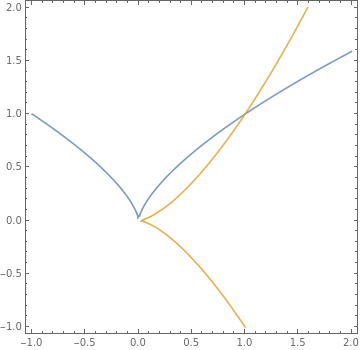
\includegraphics[width  = 4cm]{Figures/KissingCusps}
      \end{subfigure}
      \begin{subfigure}{0.45\textwidth}
        \centering
          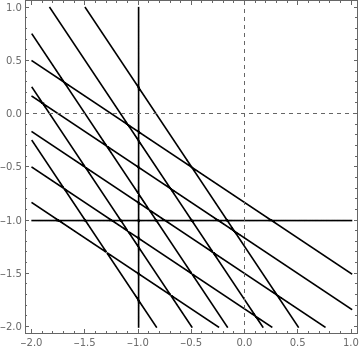
\includegraphics[width = 4cm]{Figures/2CuspsBS}
      \end{subfigure}
      \caption{On the left: the zero loci determined by $f_1(x,y) = y^2 -x^3$ and $f_2(x,y) = x^2 -y^3$ respectively in orange and blue.
      On the right: the
      Bernstein-Sato zero-locus $Z(B_F^1)$.}
      \label{fig: TwoCusps}
    \end{figure}


The first goal of this chapter is to to further refine part (1) of the above theorem by generalising Lichtin's estimate from \cref{sec: MonodromyBS}.
This means we provide a lower bound on the constant $c$ in terms of numerical data from a resolution of singularities.

Let $\mu:Y\to X$ be a strong log resolution of $f$.
The numerical data is given by the orders of vanishing $\ord_{E}(f_j)\in\mathbb{Z}_{\geq 0}$ of $f_j$ along  irreducible components $E$ of $\mu^*D$, and the orders of vanishing $k_E=\ord_{E}(\det \operatorname{Jac}(\mu))\in\mathbb{Z}_{\geq 0}$ of the determinant of the Jacobian of $\mu$, also equal to the coefficients of the relative canonical divisor $K_\mu$ of $\mu$. We show:
\begin{theorem}\label{thm: MainTheorem}
  Every irreducible component of $Z(B_F^a)$ of codimension $1$ is a hyperplane of the form
  $$\ord_{E}(f_1)s_1 + \cdots + \ord_{E}(f_r)s_r + k_E + c=0 $$
with $c\in\bZ_{>0}$.
\end{theorem}

Without the term $k_E$ the statement was proven for $r\ge 1$ by \cite[Lemma 4.4.6]{budur2020zeroII} generalising Kashiwara's estimate.
The case $r=1$ of Theorem \ref{thm: MainTheorem} is due to Lichtin \cite{lichtin1989poles}, a new proof of which was given by Dirks-Musta\c{t}\u{a} \cite{DM}.

The second part of this chapter contains a number of lower bounds for the Bernstein-Sato zero locus.
Firstly, we provide a multivariate generalisation for the fact that the Bernstein-Sato polynomial for $r=1=a$ always has the trivial root $-1$.
\begin{proposition}
  Let $E$ be an irreducible component of $D$.
  Then $\sum_{j=1}^r \ord_{E}(f_j)s_j + c = 0$ determines an irreducible component of $Z(B_F^a)$ for $c = 1,\ldots, \sum_{j=1}^{r}\ord_{E}(f_j)a_j$.
\end{proposition}
Further, we generalise the fact that the jumping numbers of $f$ in $[0,\lct(f)+1)$ are roots of $b_{f}(s)$ in the case $r=1$ \cite[Theorem 2]{BSArbitraryVariety}.
For any $\lambda\in \mathbb{R}_{\geq 0}^r$ the mixed multiplier ideal sheaf of $F^\lambda$ is given by
$$\mathcal{J}(F^\lambda) = \mu_*\O_Y(K_\mu - \lfloor \sum_{j=1}^r \lambda_j \mu^* D_j \rfloor)$$
where $D_i$ denotes the divisor determined by $f_i$ and $\lfloor \blank \rfloor$ is the round-down of an $\mathbb{R}$-divisor.
Associated to $\lambda$ is the region $$\mathcal{R}_F(\lambda):= \{\lambda'\in \mathbb{R}_{\geq 0}^r:\mathcal{J}(F^{\lambda}) \subseteq \mathcal{J}(F^{\lambda'})\}.$$

The jumping numbers from the case $r=1$ are generalised by the jumping wall associated to $\lambda$ which is the intersection of the boundary of $\mathcal{R}_F(\lambda)$ with $\mathbb{R}_{>0}^r$.
By the definition of mixed multiplier ideals the facets of the jumping wall are cut out by hyperplanes of the form
$\sum_{j=1}^r\ord_E(f_j)s_j = k_E + c$
with $c\in \mathbb{Z}_{>0}$ and $E$ an irreducible component of $\mu^*D$.
\begin{example}
  Let $f_i(x,y) = \prod_{j=1}^{n_1} \ell_{1j}$ and $f_2(x,y) = \prod_{j=1}^{n_2} \ell_{2j}$ for linear polynomials $\ell_{ij}$ which go through the origin and all have different zero loci.
  Consider a blow-up at the origin.
  For any irreducible polynomial $p\in \C[x,y]$ denote $E_p$ for the divisor determined by $p$ and denote $E_{e}$ for the exceptional divisor of the blowup.
  Then the global sections of $\mathcal{J}(F^s)$ are the polynomials $h\in \C[x,y]$ such that for all $i,j$
  $$\ord_{E_{\ell_{ij}}} h\geq \lfloor s_i \rfloor;\qquad \ord_{E_{e}} h \geq \lfloor n_1s_1 + n_2s_2 - 1 \rfloor. $$
  \begin{figure}[h!]
    \centering
    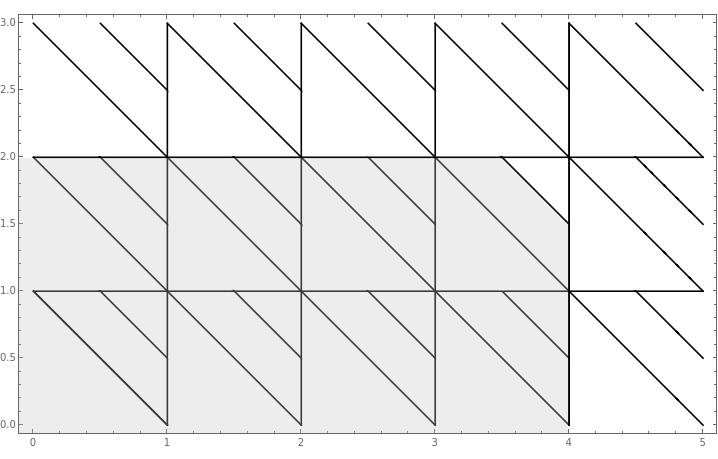
\includegraphics[width = 0.5\textwidth]{Figures/LargeJumps}
    \caption{The jumping walls and a region $\mathcal{R}_F(\lambda)$ for $f_1(x,y) =xy$ and $f_2(x,y)=(x+y)(x-y)$.}
  \end{figure}
\end{example}
The log-canonical threshold is generalised by the $\LCT$-polytope
$$ \LCT(F) :=  \bigcap_{E}\{\lambda\in \mathbb{R}_{\geq 0}^r : \sum_{j=1}^r \ord_E(f_j)\lambda_j \leq k_E + 1\}$$
where $E$ runs over the irreducible components of $\mu^*D$.
The suitable generalisation for the region $[0,\lct(f) + 1)$ is the $\KLT_{a}$-region
$$\KLT_{a}(F):= \bigcap_{E}\{\lam\in \mathbb{R}_{\geq 0}^r: \sum_{j=1}^r \ord_E(f_j)(\lambda_j - a_j) < k_E + 1\}.$$
A rephrasing in terms of being log-canonical or Kawamata log-terminal is provided in \cref{sec: JumpingWall}.
This rephrasing also shows that the regions are independent of the chosen resolution.
\begin{theorem}\label{thm: JumpingWall}
  Suppose that $\sum_{j=1}^r \ord_E(f_j)s_j = k_E + c$ determines a facet of a jumping wall which intersects $\KLT_{a}(F)$.
  Then $\sum_{j=1}^r \ord_E(f_j)s_j + k_E + c = 0$ determines a component of $Z(B_F^a)$.
\end{theorem}
This theorem was shown by \cite{cassou2011multivariable} for $Z(B_F^{1})$ when $f_1,\ldots, f_r$ are germs of plane curves.
We employ the same method, which is essentially the one used in \cite[Theorem B]{ClassicalJump} based on an idea by \cite{kollar1997singularities}.

From \Cref{thm: JumpingWall} we deduce a generalisation for the fact that the largest root of the Bernstein-Sato polynomial $b_f(s)$ is equal to the log-canonical threshold when $r=1$.
\begin{corollary}\label{thm: LCT}
  Suppose that $\sum_{j=1}^r \ord_E(f_j)s_j = k_E + 1$ determines a face of $\LCT(F)$. If $a_j\neq 0$ and $\ord_{E}(f_j)\neq 0$ for some $j$, then $\sum_j \ord_{E}(f_j)s_j +k_E + 1=0$ determines a component of $Z(B_F^a)$.
 % Moreover, if $\sum_j \ord_{E}(f_j)s_j +k_E+c = 0$ determines a codimension-one component of $Z(B_F^a)$, then $c\ge  1$.
\end{corollary}
Note that \Cref{thm: MainTheorem} implies the analogue of the maximality statement: the components of codimension one of $Z(B_F^a)$ originating from the $\LCT$-polytope are closest to the origin with that slope.

\cite{RealLogCan} also introduced a real version of jumping numbers and proved that these produce roots of the Bernstein-Sato polynomial.
Interesting about these real jumping numbers is that they do not have to agree with the complex jumping numbers.
These results are of further interest due to applications in algebraic statistics.

Mixed multiplier ideals and their jumping walls will be defined on real algebraic manifolds in \cref{sec: RealJump}.
There are also the associated notions of a $\RKLT_a$-region,  $\RLCT$-polytope and real Bernstein-Sato ideal $B_{\mathbb{R},F}^a$.
We prove the following generalisation of Saito's result on the real jumping walls.
\begin{theorem}
  Suppose that $\sum_{j=1}^r \ord_E(g_j)s_j = k_E + c$ determines a facet of a real jumping wall which intersects $\RKLT_{a}(F)$.
  Then $\sum_{j=1}^r \ord_E(g_j)s_j + k_E + c = 0$ determines a component of $Z(B_{\mathbb{R},F}^a)$.
\end{theorem}

\section{$\D_X[s]$-modules}\label{sec: DXS}
This section provides preliminaries on the theory of $\D_X[s]$-modules, such as direct images and homological properties.

\subsection{Relative holonomic $\sD$-modules}\label{sec: RelHol}
Let $X$ be a smooth complex variety and let $R$ be a regular commutative finitely generated $\C$-algebra integral domain. The sheaf of relative differential operators on $X$ is defined by
$$\D_X^R := \D_X \otimes_\C R.$$
The order filtration $F_j \D_X$ on $\D_X$ extends to a filtration $F_j \D_X^R := F_j\D_X\otimes_\C R$ on $\D_X^R$.
The graded objects for this filtration are denoted by $\grrel$.
Denote $\pi_{T^*X}:T^*X \to X$ for the projection map.
Recall from \cref{sec: SheafOfDiff} that $\gr\D_X \cong \pi_* \O_{T^*X}$, it follows that $\grrel\D_X^R \cong (\pi_{T^* X}\times \pi_{\Spec R})_*\O_{T^*X\times \Spec R}$ for $\pi_{\Spec R}: \Spec R \to \{\operatorname{pt}\}$ the projection onto a point.


Since $\D_X^R$ is a sheaf of non-commutative rings, one should distinguish between left and right $\D_X^R$-modules.
We may also refer to a $\D_X^R$-module without specifying left or right if no confusion is possible. In these cases it is intended that the result holds in either case.

For any filtered $\D_X^R$-module $\M$ there is an associated sheaf of modules on $T^*X\times \Spec R$ given by
$(\pi\times \Id_{\Spec R})^{-1}(\grrel\M)\allowbreak\otimes_{\pi^{-1}\grrel\D_X^R} \O_{T^*X\times \Spec R}$.
From here on out we write $\grrel\D_X^R$ and $\grrel \M$ for the corresponding sheaves on $T^*X\times \Spec R$.

A filtration  compatible with $F_\bullet \sD_X^R$ on a $\D_X^R$-module $\M$ is said to be good if $\grrel\M$ is a coherent $\grrel\D_X^R$-module.
A quasi-coherent $\D_X^R$-module $\M$ locally admits a good filtration if and only if it is coherent \cite[Corollary D.1.2]{hotta2007d}, in fact one can take this filtration to be global \cite[Proof of Theorem 2.1.3]{hotta2007d}.
For a coherent $\D_X^R$-module $\M$ the support $\Chrel\M$ of $\grrel\M$ in $T^*X\times \Spec R$ is independent of the chosen filtration \cite[Lemma D.3.1.]{hotta2007d} and is called the relative characteristic variety.
Equivalently, the relative characteristic variety is locally determined by the radical of the annihilator ideal of $\grrel \M$ in $\grrel\D_X^R$.
\begin{proposition}{\cite[Lemma 3.2.2]{budur2020zeroI}}\label{prop: SESBehaviourChrel}
  For any short exact sequence of coherent $\D_X^R$-modules
  $$0\to \M_1\to \M_2 \to \M_3 \to 0 $$
  it holds that $\Chrel\M_2 = \Chrel\M_1 \cup \Chrel\M_3.$
\end{proposition}
\begin{definition}\label{def: RelHolonomic}
  A coherent $\D_X^R$-module $\M$ is said to be relative holonomic if its characteristic variety is a finite union $\Chrel\M = \cup_w \Lambda_w \times S_w$ where $\Lambda_w\subseteq T^* X$ are irreducible conic Lagrangian subvarieties and $S_w\subseteq \Spec R$ are irreducible subvarieties.
\end{definition}

\begin{proposition}{\cite[Lemma 3.2.4]{budur2020zeroI}}\label{prop: SubquotientRelHol}
  Any subquotient of a relative holonomic module is relative holonomic.
\end{proposition}
%It is necessary to distinguish between left and right $\D_X^R$-modules since the rings $\D_X^R$ are non-commutative.
%Whenever a result applies to both left and right $\D_X^R$-modules we will simply refer to a $\D_X^R$-module.
%A module which is equipped with both structures is called a $\D_X^R$-bimodule.
%In particular, for any ideal $I\subseteq R$ the ideal sheaf $\D_X^{R/I}$ may be viewed as a $\D_X^R$-bimodule.

%Giving a left $\D_X^R$-module is equivalent to giving a $\O_X^R$-module $\M$ with a $\Theta_X$-action such that $\xi\cdot(fm)=f(\xi\cdot m) + \xi(f)$ for any section $f$ of $\O_X$ and vector field $\xi$.
%Similarly, giving a right $\D_X^R$-module is equivalent to giving a $\O_X^R$-module $\M$ with a $\Theta_X$-action such that
%$(mf)\cdot \xi = (m\cdot \xi)f - m\xi(f)$.

The functor which associates to a left $\D_X^R$-module $\M$ the right $\D_X^R$-module $\M\otimes_{\O_X}\omega_X$ is an equivalence of categories.
The pseudoinverse associates $\Hom_{\O_X}(\omega_X,\allowbreak\M)$ to a given right-module $\M$.

Pick local coordinates $x_1,\ldots, x_n$ on $X$, these are regular functions such that is to say that $dx_1,\ldots,dx_n$ are a local basis for $\Omega_{X}^1$.
There is an induced section $dx := dx_1\wedge \ldots \wedge dx_n$ for $\omega_X$.

For any left $\D_X^R$-module $\M$ one now gets a locally defined $\O_X\otimes R$-linear isomorphism $\M \to \M\otimes_{\O_X}\omega_X$  associating to any section $m$ the section $m^* = m dx$.
This can be made to commute with the $\D_X^R$-module structure.
This is to say that for any operator $P$ of $\D_X^R$ there is an adjoint $P^*$ such that
$$(P\cdot m)^* = m^* \cdot P^*.$$
Indeed, for a vector field $\xi = \sum \xi_i \partial_i$ this is satisfied by setting $\xi^* = -\sum \partial_i \xi_i$.
Iteration then extends to differential operators of arbitrary order.
\subsection{Direct image}
Let $\mu:Y\to X$ be a morphism of varieties.
The direct image functor $\int \M:= R\mu_*(\M\otimes_{\D_Y}^L \D_{Y\to X}) $ on right $\D_Y$-modules induces an $\D_Y^R$-module direct image functor.
Indeed, consider a right $\D_Y^R$-module $\M$ and observe that multiplication by $r\in R$ is $\D_Y$-linear.
By the functoriality of the $\D_Y$-module direct image it follows that there is an associated endomorphism on $\int \M$.
This equips the direct image with a canonical structure as complex of $\D_X^R$-modules.
For any $j\in \mathbb{Z}$ we still call $\int^j\M := H^j\int\M$ the $j$-th direct image.

Whenever $\mu$ is proper and $\M$ is coherent as $\D_Y^R$-module it holds that $\int^j\M$ is coherent over $\D_X^R$ for any $j$.
The proof for this statement is identical to the absolute case \cite[Theorem 2.5.1]{hotta2007d}.
The following proposition may be established identically to the absolute case which was established in \cref{cor: RelHolConserved}.
\begin{proposition}\label{prop: DirectImageRelHol}
  Suppose that $\mu$ is proper and let $\M$ be a relative holonomic right $\D_Y^R$-module.
  Then $\int^j \M$ is relative holonomic for any $j\in \mathbb{Z}$.
\end{proposition}
%an analytical version of this result may be found in  \cite[Theorem 1.17]{monteiro2016riemann}.
\subsection{Homological notions}\label{sec: HomNotion}
In this section it is assumed that $X$ is affine. We denote $n = \dim X$ and $r = \dim R$ for the Krull dimension of the ring $R$.
For some results in this section the distinction between left and right modules is relevant.
Such results have been stated in terms of right $\D_X^R$-modules, which is the case we will need. It should be clear that these results have obvious analogues for left $\D_X^R$-modules.


\subsubsection{Grades}
\begin{definition}
  Let $\M$ be a non-zero coherent $\D_X^R$-module. The smallest integer $j\geq 0$ such that $\Ex{\D_X^R}{j}(\M,\D_X^R) \neq 0$ is called the grade of $\M$ and is denoted $j(\M)$. If $\M = 0$ then $j(\M)$ is said to be infinite.
\end{definition}
\begin{remark}
  Observe that $\Ext$ localises. This is to say that for any localisation $R'$ of $R$ $$\Ex{\D_X^R}{j}(\M,\D_X^R)\otimes_R R' \cong \Ex{\D_X^{R'}}{j}(\M\otimes_R R',\D_X^{R'}).$$
  Hence, $j(\M)\leq j(\M\otimes_R R')$.
\end{remark}
\begin{definition}\label{def: BSIdeal}
  The Bernstein-Sato-ideal of a $\D_X^R$-module $\M$ is given by $B_\M:=\Ann_R \M$.
\end{definition}

\begin{proposition}[{\cite[Lemma 3.4.1]{budur2020zeroI}}]\label{prop: ChrelGrades}
  Let $\M$ be a relative holonomic $\D_X^R$-module then
  $$\dim \Chrel \M + j(\M) = 2n + r.$$
\end{proposition}
\begin{remark}\label{rem: GradeIFFBernsteinIdeal}
  Further \cite[Lemma 3.2.2]{budur2020zeroI} states that $Z(B_\M)$, the reduced closed subscheme defined by the radical ideal of $B_\M$ in $\Spec R$, is the projection of $\Chrel\M$ on $\Spec R$.
  Hence, $j(\M)=n+k$ for a relative holonomic module $\M$ if and only if $Z(B_\M)$  has codimension $k$ in $\Spec R$.
  \end{remark}
\begin{definition}
  A non-zero coherent $\D_X^R$-module $\M$ is said to be $j$-pure if $j(\N) = j(\M) = j$ for every non-zero submodule $\N$.
\end{definition}
\begin{proposition}[{\cite[Lemma 4.3.5.]{budur2020zeroI}}]\label{prop: JPureExt}
   Let $\M$ be a non-zero coherent right $\D_X^R$-module of grade $j$. Then:
\begin{enumerate}
\item    $\Ex{\D_X^R}{j}(\M,\D_X^R)$ is a $j$-pure left $\D_X^R$-module and $\Ex{\D_X^R}{k}(\M,\D_X^R)$ has grade $\ge k$ for any $k\neq j$;
\item $\M$ is $j$-pure if and only if $\Ex{\D_X^R}{k}(\Ex{\D_X^R}{k}(\M,\D_X^R),\D_X^R)= 0$ for every $k\neq j$.
\end{enumerate}
 \end{proposition}
 \begin{proposition}[{\cite[Lemma 3.4.2]{budur2020zeroI}}]\label{prop: Injective3.4.2}
   Let $\M$ be a $j$-pure relative holonomic $\D_X^R$-module and suppose that $b\in R$ is not contained in any minimal prime ideal of $R$ containing $B_\M$. Then there exists a good filtration on $\M$ such that multiplication by $b$ induces injective endomorphisms on $\M$ and $\grrel\M$.
 \end{proposition}
 \begin{proposition}[{\cite[Lemma 3.2.4.]{budur2020zeroI}}]
   Let $\M$ be a relative holonomic right $\D_X^R$-module. Then, for any $k\geq 0$, $\Ex{\D_X^R}{k}(\M,\D_X^R)$ is a relative holonomic left $\D_X^R$-module.
 \end{proposition}
 \begin{proposition}\label{prop: TorRelHol}
   Let $\M$ be a relative holonomic right $\D_X^R$-module and let $P\subseteq R$ be a prime ideal with $Z(P)$ non-singular. Then, for any $k\geq 0$, $\Tr{\D_X^R}{k}(\M,\D_X^{R/P})$ is a relative holonomic right $\D_X^{R/P}$-module.
 \end{proposition}
 \begin{proof}
   The assumption on $P$ is equivalent to assuming that $R/P$ is a ring of the same type as $R$, namely a commutative regular finitely generated $\bC$-algebra integral domain.
   Let $\mathcal{F}^\bullet$ be a resolution of $\D_X^{R/P}$ by free $\D_X^R$-bimodules of finite rank.
   Then $\Tr{\D_X^R}{k}(\M, \allowbreak\D_X^{R/P})$ is found from the cohomology of the complex $\M\otimes_{\D_X^R}\mathcal{F}^{\bullet}$.
   The entries of this complex remain relative holonomic so
   \Cref{prop: SubquotientRelHol} shows that $\Tr{\D_X^R}{k}(\M,\D_X^{R/P})$ is a relative holonomic right $\D_X^R$-module.

   This means that $\Tr{\D_X^R}{k}(\M,\D_X^{R/P})$ admits a good filtration such that $$\supp \gr_{\D_X^R}^{rel}\Tr{\D_X^R}{k}(\M,\D_X^{R/P}) = \cup_w \Lambda_w \times S_w $$
   for Lagrangian subvarieties $\Lambda_w\subseteq T^*X\times \Spec R$ and algebraic varieties $S_w \subseteq \Spec R$.
   This filtration descends to a good filtration over $\D_X^{R/P}$ and it holds that
   $$\supp \gr_{\D_X^{R/P}}^{rel} \Tr{\D_X^R}{k}(\M,\D_X^{R/P}) = (\Id_{T^*X}\times \Delta)^{-1}(\supp \gr_{\D_X^R}^{rel}\Tr{\D_X^R}{k}(\M,\D_X^{R/P}))$$
   where $\Delta: \Spec R/P\to \Spec R$ is the closed embedding.
   This proves the desired result.
 \end{proof}
 \begin{proposition}{\cite[Corollary 5.8.4]{weibel1995introduction}}
   For any coherent right $\D_X^R$-module $\M$ and prime ideal $P\subseteq R$ with $Z(P)\subseteq \Spec R$ non-singular there is a spectral sequence
  $$E_2^{pq}= \Ex{\D_X^{R/P}}{p}(\Tr{\D_X^R}{-q}(\M,\D_X^{R/P}), \D_X^{R/P}) $$
  converging to $H^{p+q}(R\Hom_{\D_X^{R/P}}(\M\otimes_{\D_X^R}^L \D_X^{R/P},\D_X^{R/P})).$
 \end{proposition}
 \begin{proof}
   This is simply the Grothendieck spectral sequence for this composition of derived functors.
   It is applicable since $\blank \otimes_{\D_X^{R}}\D_X^{R/P}$ transforms projective right $\D_X^R$-modules into projective right $\D_X^{R/P}$-modules and these are acyclic for $\Hom_{\D_X^{R/P}}(\blank,\D_X^{R/P})$.
 \end{proof}

 \begin{proposition}
   For any coherent right $\D_X^R$-module $\M$ and right $\D_X^R$-module $\N$ there is a spectral sequence
   $$E_2^{pq}= \Tr{\D_X^R}{-p}(\N,\Ex{\D_X^R}{q}(\M,\D_X^R)) $$
   converging to $H^{p+q} (\N\otimes_{\D_X^R}^L R\Hom_{\D_X^R}(\M,\D_X^R) ).$
 \end{proposition}
 \begin{proof}
   The conditions of the Grothendieck spectral sequence \cite[Corollary 5.8.4]{weibel1995introduction} are not satisfied in this case.
   For instance, $\Hom_{\sc{\D_X^R}}(\blank,\D_X^R)$ does not necessarily transform projective objects into $(\N\otimes_{\D_X^R}\blank)$-acyclic objects.
   Still, the same proof applies with some minor modifications.

  Take a resolution $\F^\bullet \to \M$ by free right $\D_X^R$-modules of finite rank.
  Let $\mathscr{P}^{\bullet\bullet}\to \Hom_{\D_X^R}(\F^{\bullet},\D_X^R)$ be the Cartan-Eilenberg resolution provided by \cref{prop: Cartan-Eilenberg}.
  It is known that any coherent left $\D_X^R$-module admits a projective resolution of length $\leq 2n + r$ \cite[p6]{budur2020zeroI}.
  Using this fact in the construction of the Cartan-Eilenberg resolution allows one to assume that $\mathscr{P}^{pq}=0$ for $-p>2n + r$.

  Consider the double complex $\N\otimes_{\D_X^R}\mathscr{P}^{\bullet \bullet}$.
  The total cohomology of this double complex comes equipped with two filtrations one vertical and one horizontal.
  These filtrations are bounded due to the bounds on $p$ so \cref{prop: FiltrationSpectral} is applicable and yield two spectral sequences converging to the total cohomology.
  The first spectral sequence has
  $$E_{2}^{pq} = H^p_h(H^q_v(\N \otimes_{\D_X^R}\mathscr{P}^{\bullet \bullet})).$$
  Observe that $\Hom_{\D_X^R}(\F^q, \D_X^R)$ is a free left module due to $\F^q$ being free of finite rank.
  In particular, these are acyclic for $(\N\otimes_{\D_X^R}\blank)$.
  Since $\mathscr{P}^{\bullet q}\to \Hom_{\D_X^R}(\F^q,\D_X^R)$ is a quasi-isomorphism it follows that $E_2^{pq}=0$ for any $p>0$ and $E_2^{0q} = H^{q} (\N\otimes_{\D_X^R}^LR\Hom_{\D_X^R}^p(\M,\D_X^R) )$.

  The other spectral sequence has
  \begin{align*}
      E_2^{pq} &= H^q_v(H^p_h(\N\otimes_{\D_X^R}\mathscr{P}^{\bullet\bullet}))\\
      &=  \Tr{\D_X^R}{-p}(\N,\Ex{\D_X^R}{q}(\M,\D_X^R))
  \end{align*}
  where it was used that the image and cohomology of the horizontal differentials are projective by the structure of the Cartan-Eilenberg resolution.

  Both spectral sequences converge to the same total cohomology.
  Since the first spectral sequence collapses on the second sheet this means that $\Tr{\D_X^R}{-p}(\N,\Ex{\D_X^R}{q}(\M,\D_X^R))$ converges to $H^{p+q}( \N\otimes_{\D_X^R}^LR\Hom_{\D_X^R}(\M,\D_X^R) )$.
 \end{proof}
 The proof of the following proposition is based on the proof of \cite[Proposition 3.4.3]{budur2020zeroI}.
 An alternative proof, based on the purifications, has been provided by van der Veer and will appear in a forthcoming paper.
 \begin{proposition}\label{prop: RestrictConservesGraden}
   Let $\M$ be a non-zero relative holonomic right $\D_X^R$-module of grade $n$.
   Then, for any $b\in R$ with $Z(b)$ non-singular and irreducible it holds that $\M\otimes_R R/(b)$ is a non-zero relative holonomic right $\D_X^{R/(b)}$-module of grade $n$.
 \end{proposition}\begin{proof}
   Applying \Cref{prop: TorRelHol} with $k=0$ yields that $\M \otimes_R R/(b)$ is a relative holonomic right $\D_X^{R/(b)}$-module.

  It remains to establish that $\M \otimes_R R/(b)$ is non-zero of grade $n$.
  By consideration of a resolution of $\M$ by free right modules of finite rank one has that
  $$ \D_X^{R/(b)} \otimes_{\D_X^R}^LR\Hom_{\D_X^R}(\M,\D_X^R) \cong R \Hom_{\D_X^{R/(b)} }(\M\otimes_{\D_X^R }^L \D_X^{R/(b)}, \D_X^{R/(b)}) $$
  where we note that $\D_X^{R/(b)}$ is a $\D_X^{R}$-bimodule so that both tensor products are well-defined.
  We compare the spectral sequences of both sides of this isomorphism.

  The spectral sequence associated with the right-hand-side has $E_2$-sheet
  $$E^{p,q}_2 = \Ex{\D_X^{R/(b)}}{p}(\Tr{\D_X^R}{-q}(\M, \D_X^{R/(b)}), \D_X^{R/(b)}).$$
  Recall from \Cref{prop: JPureExt} that terms with $p>n$ have grade greater than $n$ and due to \Cref{prop: ChrelGrades} there are no non-zero terms with $p<n$.
  Hence, the only term with $p+q = n$ which could potentially have grade $n$ is $E^{n,0}_2$.
  It now suffices to show that the total cohomology of degree $n$ on the left-hand-side has grade $n$.
  Indeed, both spectral sequences must have the same limit and due to \Cref{prop: ChrelGrades} and \Cref{prop: SESBehaviourChrel} the total cohomology of degree $n$ can only have grade $n$ if some $E^{p,q}_\infty$-term with $p+q=n$ has grade $n$.
  Again by \Cref{prop: ChrelGrades} and \Cref{prop: SESBehaviourChrel} this is only possible if some $E^{p,q}_2$-term has grade $n$.

  The spectral sequence associated to the left-hand-side has $E_2$-sheet given by
  $$E_2^{p,q} =\Tr{\D_X^R}{-p}(\D_X^{R/(b)}, \Ex{\D_X^R}{q}(\M,\D_X^R)).$$
  Note that there are no non-zero differentials out of $E_j^{0,n}$ for $j\geq 2$.
  Further, the differentials into $E^{0,n}_j$ stem from $E^{-j,(n+j-1)}_j$ which is a subquotient of $\Tr{\D_X^R}{j}( \D_X^{R/(b)} ,\Ex{\D_X^R}{n+j-1}(\M, \D_X^R))$.
  Observe that $\D_X^R \xrightarrow{b} \D_X^R $ yields a free resolution for $\D_X^{R/(b)}$.
  It follows that $E^{-j,(n+j-1)}_j=0$ for $j\geq 2$ whence $E_j^{0,n} = E_2^{0,n}$ for all $j\geq 2$.
  It remains to show that that $E_2^{0,n}$ has grade $n$.

  Denote $\E^n := \Ex{\D_X^R}{n}(\M,\D_X^R)$, by \Cref{prop: JPureExt} $\E^n$ is a $n$-pure relative holonomic left $\D_X^R$-module.
  By \Cref{rem: GradeIFFBernsteinIdeal} we have that $B_{\E^n}=0$, in particular $b$ does not belong to any minimal prime ideal containing $B_{\E^n}$.
  Hence, by \Cref{prop: Injective3.4.2}, $\E^{n}$ admits a good filtration such that $b$ induces injections on $\E^{n}$ and $\gr^{rel} \E^{n}$.
  In particular the vertical maps in the following diagram are injective
  $$\begin{tikzcd}
    0 \arrow{r} & F_{i-1} \E^n\arrow{r} \arrow{d}{b}& F_i \E^{n}\arrow{r} \arrow{d}{b}& \gr^{rel}_i \E^n\arrow{r}\arrow{d}{b} & 0\\
    0 \arrow{r} & F_{i-1} \E^n\arrow{r} & F_i \E^{n}\arrow{r} & \gr^{rel}_i \E^n\arrow{r} & 0
  \end{tikzcd} $$
  so the snake lemma yields a short exact sequence
  $$\begin{tikzcd}
    0 \arrow{r} & R/(b)\otimes_R F_{i-1} \E^n\arrow{r} & R/(b)\otimes_R F_i \E^{n} \arrow{r} & \arrow{r}R/(b)\otimes_R \gr^{rel}_i \E^n & 0.
  \end{tikzcd} $$
  The injectivity of $b$ on $\gr^{rel}\E^n$ implies that $b$ is also injective on $\E^n/F_i\E^n$. A similar application of the snake lemma now yields a short exact sequence
  $$\begin{tikzcd}
    0 \arrow{r} &R/(b) \otimes_R F_{i} \E^n\arrow{r} & R/(b)\otimes_R \E^{n}\arrow{r} & \arrow{r} R/(b)\otimes_R(\E^n/F_i \E^n ) & 0.
  \end{tikzcd} $$
  A filtration on $R/(b) \otimes_R \E^n$ is induced by the image of $F_i\E^n$. By the injectivity of the second short exact sequence one now has isomorphisms
  \begin{align*}
    F_i( R/(b)\otimes_R\E^n ) \cong F_i\E^n / (F_i \E^n \cap b\E^n) \cong F_i \E^n / b F_i \E^n \cong   R/(b)\otimes_R (F_i\E^n)
  \end{align*}
  combined with the surjectivity of the first short exact sequence it follows that
  $$\gr^{rel}(R/(b) \otimes_R \E^n) \cong  R/(b)\otimes_R \gr^{rel}\E^n. $$
  It follows that
  $$\Ch^{rel}(\D_X^{R/(b)}\otimes_{\D_X^R} \E^n )  = (\Id_{T^*X} \times \Delta)^{-1}(\Chrel \E)$$
  with $\Delta: \Spec R/(b) \to \Spec R$ the closed embedding as before.
  Since $\E^n$ has grade $n$ this equality and \Cref{prop: ChrelGrades} imply that $\Ch^{rel}(\D_X^{R/(b)} \otimes_{\D_X^R} \E^n)$ has dimension $n + r - 1$.
  In particular it follows that $\D_X^{R/(b)} \otimes_{\D_X^R}\E^n $ is non-zero and has grade $n$. This concludes the proof.
 \end{proof}
\subsubsection{Relative Cohen-Macaulay $\sD$-modules}
 \begin{definition}[\cite{{budur2020zeroI}}]
   A coherent $\D_X^R$-module $\M$ is said to be $j$-Cohen-Macaulay for some $j\geq 0$ if $\Ex{\D_X^R}{k}(\M,\D_X^R) = 0$ for any $k\neq j$.
 \end{definition}
 \begin{remark}
  If $\M$ is $j$-Cohen-Macaulay then, by \Cref{prop: JPureExt}, it is $j$-pure.
 \end{remark}
 \begin{proposition}{\cite[Proof of Proposition 3.4.3]{budur2020zeroI}}\label{prop: CMRestriction}
   Let $\M$ be a relative holonomic and $(n+k)$-Cohen-Macaulay right $\D_X^R$-module. Let $b\in R$ be a prime element such that $Z(b)$ is non-singular and does not contain any irreducible component of $Z(B_\M)$. Then it holds that $\M\otimes_R R/(b)$ is a relative holonomic and $(n+k)$-Cohen-Macaulay right $\D_X^{R/(b)}$-module or zero.
 \end{proposition}
 \begin{proposition}{\cite[Proof of Proposition 3.5.2]{budur2020zeroI}}\label{prop: RestrictToCM}
   Let $\M$ be a relative holonomic right $\D_X^R$-module of grade $n+k$ and $V\subseteq \Spec R$ be a variety with irreducible components of codimension $\leq k$.
   Then there exists an affine open $\Spec R' \subseteq \Spec R$ such that $\M\otimes_R R'$ is a relative holonomic and $(n+k)$-Cohen-Macaulay right $\D_X^{R'}$-module.
    Moreover, it may be assumed that $\Spec R'$ intersects every irreducible component of $V$.

    Similarly, if $\M$ is relative holonomic of grade $>n+k$ and $V\subseteq \Spec R$ is a variety with irreducible components of codimension $\leq k$ then there exists an affine open $\Spec R'\subseteq \Spec R$ such that $\M\otimes_R R' = 0$ and $\Spec R'$ intersects every irreducible component of $V$.
 \end{proposition}

 \section{Upper bound for the Bernstein-Sato zero locus}\label{sec: UpperBound}
 Since $B_F^a$ is the intersection of all local $B_{F,x}^a$ it is sufficient to establish \Cref{thm: MainTheorem} locally.
 Hence, without loss of generality, we may assume that $X$ is affine and admits local coordinates $x_1,\ldots, x_n$.
 Recall from the introduction that $G = F\circ\mu$ and denote $g_j$ for the coordinate functions of $G$.
 \subsection{Translation to right-module}
 By the translation between left and right modules in \Cref{sec: RelHol} the functional equation $P F^{s+a} = b F^s$ may be restated as the equation
 $$F^{s+a}dx \cdot P^* = b F^s dx $$
 in $\D_X^{\C[s]} F^s \otimes_{\O_X}\omega_X$.
 Define $\M$ to be the submodule of $ \D_Y^{\C[s]} G^s\otimes_{\O_Y}\omega_Y$ spanned by $G^s \mu^*(dx)$ over $\D_Y^{\C[s]}$.
 \begin{lemma}
   The right $\D_Y^{\C[s]}$-module $\M$ is relative holonomic.
 \end{lemma}
 \begin{proof}
   The left $\D_Y^{\C[s]}$-module $\D_Y^{\C[s]}G^s$ is relative holonomic following \cite[Result 1]{maisonobe2016filtration}.
   Then the associated right-module $\D_Y^{\C[s]}G^s\otimes_{\O_Y} \omega_Y$ is also relative holonomic.
   Hence, \Cref{prop: SubquotientRelHol} implies that the submodule $\M$ is also relative holonomic.
 \end{proof}
 \subsection{$\D_X\langle s, t\rangle$-modules}
 Let $\D_X\langle s,t \rangle$ denote the sheaf of rings found from $\D_X^{\C[s]}$ found by adding a new variable $t$ which commutes with sections of $\D_X$ and is subject to $s_j t = t(s_j +a_j)$ for every $j=1,\ldots, r$ .
 The $\D_X^{\C[s]}$-module $\D_X^{\C[s]} F^s\otimes_{\O_Y}\omega_Y$ may be equipped with the structure of a right $\D_X\langle s, t\rangle$-module by the action
 $$F^sdx P(x,\partial,s) \cdot t  =F^{s + a}dx P(x,\partial, s + a).$$
 In this formalism $B_F^a$ is the Bernstein-Sato ideal of $(\D_X^{\C[s]} F^s\otimes_{\O_Y}\omega_Y) / (\D_X^{\C[s]} F^s\otimes_{\O_Y}\omega_Y) t$.
 An analogous $\D_Y\langle s,t\rangle$-module structure can be given to $\M$.
 \begin{lemma}\label{lem: BernsteinSatoPolynomialUpstairs}
  The Bernstein-Sato ideal $B_{\M/\M t}$ contains a polynomial of the form
  $$b(s)=\prod_E \prod_{j=1}^N(\ord_{E}(g_1) s_1 + \cdots + \ord_{E}(g_r) s_r + k_i + j)$$
  where $E$ ranges over the irreducible components of $\mu^*D$ and $N\in \mathbb{Z}_{\geq 0}$.
 \end{lemma}
 \begin{proof}
  This follows from a local computation which is analogous to the corresponding local computation in  of \cite[Section 4]{lichtin1989poles}.
 Suppose we are working near a point $y\in Y$ which is on the irreducible component $E_i$ of $\mu^*D$ if and only if $i\in I$.
 Pick local coordinates $z_1,\ldots,z_n$ where every $E_i$ with $i\in I$ is determined by some $z_{j_i}$.
 After relabeling the $E_i$ it may be assumed that $j_i = i$.

 In these local coordinates
 $$G^s = \prod_{j=1}^r u_j^{s_j} \prod_{i\in I} z_i^{\sum_{j=1}^r   \ord_{E_i}(g_j)s_j};\qquad \mu^*(dx) = v \prod_{i\in I} z_i^{k_i} dz$$
 where $u_j, v$ are local units.
 For any $i\in I$ set $\xi_i := -\partial_i - \sum_{j=1}^{r}s_j\partial_j(u_j)u_j^{-1}$ and let $P = v^{-1}(\prod_{j=1}^r u_j^{-a_j}) (\prod_{i\in I}\xi_i^{\sum_{j=1}^r a_j\ord_{E_i}(g_j)}) v$ then
 $$G^{s+a}\mu^*(dx) \cdot P =  q(s) G^s \mu^*(dx) $$
 where
 $$q(s) = \prod_{i\in I}((\sum_{j=1}^r \ord_{E_i}(g_j)s_j + a_j\ord_{E_i}(g_j)) + k_i)\cdots((\sum_{j=1}^r \ord_{E_i}(g_j)s_j) + 1 + k_i ).$$
 \end{proof}
 \subsection{Coherence as $\D_Y$-module}
  The goal of this section is to show that it may be assumed that $\M$ is coherent as a $\D_Y$-module.

  Pick $r$ independent linear polynomials $\sum_{j=1}^r d_{ij}s_j$ such that for any $i=n+1,\ldots,n+r$ there is no hyperplane parallel to $\sum_{j=1}^r d_{ij}s_j = 0$ in $Z(B_{F,x}^a)$ and the $d_{ij}$ are non-negative integers.
  Introduce new coordinates $z_{n+1}, \ldots,z_{n+r}$ and set $\widetilde{f}_j = f_j\prod_{i=n+1}^{n+r} \allowbreak z_{i}^{d_{ij}}$ on $X\times \C^r$.
  Note that the induced map $Y\times \C^r \to X\times \C^r$ is a resolution of singularities for $\prod \widetilde{f}_i$ and that $\widetilde{g}_j = g_j\prod_{i=n+1}^{n+i} z_{i}^{d_{ij}}$ is the pullback of $\widetilde{f}_i$.

  For any $i=n+1,\ldots,n+r$ consider the action of $\partial_{i}$ on the generator
  $$\widetilde{G}^s \mu^*(dx)\cdot \partial_{i} = -\sum_{j=1}^r d_{ij}s_j z_{i}^{-1} \widetilde{G}^s \mu^*(dx).$$
  Recall that the $\sum_{j=1}^r d_{ij}s_j$ are independent by assumption.
  It follows that an appropriate $\C$-linear combination of the vector fields $\partial_{i}z_{i}$ provides a vector field $\mathcal{S}_j$ acting as $s_j$ on the generator.
  Hence, coherence as a $\D_{Y\times \C^r}^{\C[s]}$-module implies the coherence as a $\D_{Y\times \C^r}$-module.
  \begin{lemma}\label{lem: ReplacementIsAllowed}
    For any $(x,p) \in X\times \C^r$ it holds that if $b\in B_{\widetilde{F},(x,p)}^a$ then $b \in B_{F,x}^a$.
  \end{lemma}
  \begin{proof}
    Take local coordinates $z_1,\ldots, z_{n+r}$ near $(x, p)$ and let $P$ be in the stalk of $\D_{X\times \C^r}^{\C[s]}$ at $(x ,p)$ such that $b \widetilde{F}^s = P \widetilde{F}^{s+a}$.

    Similarly to the above there exists a $\C$-basis $\zeta_1,\ldots,\zeta_r$ for the span of $\partial_{n+1}, \ldots, \partial_{n+r}$ so that $\mathcal{S}_j' := z_{n+j}\zeta_j$ satisfies $\mathcal{S}_j \cdot \widetilde{F}^s = s_{j}\widetilde{F}^s$.
    Expand $P$ as a polynomials in $\zeta_1,\ldots,\zeta_r$
    $$P = \sum_{\alpha} P_\alpha \zeta_{1}^{\alpha_1}\cdots \zeta_{r}^{\alpha_r}$$
    where the coefficients $P_\alpha$ live in the stalk of $\O_{X\times \C^r}\otimes_{\O_{X}}\D_{X}^{\C[s]}$ at $(x,p)$.

    Let $N$ be greater than the maximal value of $\abs{\alpha}$ then
    $$(z_{n+1}\cdots z_{n+r})^N b \widetilde{F}^s = \left(\sum_{\alpha} \prod_{i=1}^r (s_i + a_i)^{\alpha_i} \sum_\beta Q_{\alpha\beta} \partial_1^{\beta_1}\cdots \partial_n^{\beta_n} \right)\widetilde{F}^{s+a}$$
  where the $P_\alpha$ were expanded as polynomials in $\partial_1,\ldots,\partial_n$ with coefficients $Q_{\alpha\beta}$ from the stalk of $\O_{X\times \C^r}$.
  Observe that $\partial_1,\ldots, \partial_n$ act on the formal symbol $\widetilde{F}^{s+a}$ the same as they act on the formal symbol $F^{s+a}$.

  Now consider this functional equation on the analytification of $X\times \C^r$ and expand $(z_{n+1}\cdots z_{n+r})^N$ and the $Q_{\alpha\beta}$ as power series at $p$.
  Identifying powers of $(z_{n+1}-p_{1})\cdots (z_{n+r} - p_r)$ on both sides a functional equation with analytical coefficients for $F^s$ follows.
  This establishes that $b$ is in the analytic Bernstein-Sato ideal.
  It follows that $ b\in B_{F,x}^a$ since analytic and algebraic Bernstein-Sato ideals agree \cite{brianccon2002remarques}.
  \end{proof}
  Replacing $F$ by $\widetilde{F}$ leaves the estimate unchanged up to hyperplanes parallel to $\sum_{j=1}^r d_{ij}s_j = 0$.
  These are not in $Z(B_{F,x}^a)$ by assumption so, by \Cref{lem: ReplacementIsAllowed}, it remains to prove the theorem for $\widetilde{F}$.
  For notational simplicity we write $F$ instead of $\widetilde{F}$ and $X$ instead of $X\times \C^r$ which has dimension $m = n + r$.
  \subsection{Reduction of the number of variables}
  Let $\ell_1,\ldots,\ell_{r-1}\in \C[s]$ be degree one polynomials which will be fixed later.
  For any $i=0\ldots,r-1$ let $L_i$ be the ideal of $\C[s]$ generated by $\ell_1,\ldots,\ell_i$.
  Assume that the $\ell_i$ are chosen sufficiently generically so that $Z(L_{r-1})$ is a line.
  \begin{proposition}\label{prop: CharVarEstimateW}
    The $\D_Y$-module $\M\otimes_{\C[s]}\C[s]/L_{r-1}$ is coherent and its (non-relative) characteristic variety satisfies $\Ch\M\otimes_{\C[s]}\C[s]/L_{r-1} \subseteq \Lambda \cup W $ where $\Lambda$ is isotropic and $W$ is an irreducible variety of dimension $m +1$ which dominates $Y$.
\end{proposition}
\begin{proof}
  The coherence of $\M\otimes_{\C[s]}\C[s]/L_{r-1}$ is immediate from the coherence of $\M$ as $\D_Y$-module.

  Let $s_0$ denote a new variable so that $\C[s]/L_{r-1}\cong \C[s_0]$. As in the proof of \Cref{lem: BernsteinSatoPolynomialUpstairs} we may pick local coordinates such that
  $$G^s = \prod_{j=1}^r u_j^{s_j} \prod_{i\in I} z_i^{\sum_{j=1}^r   \ord_{E_i}(g_j)s_j};\qquad \mu^*(dx) = v \prod_{i\in I} z_i^{k_i} dz$$
  where $u_j, v$ are local units and we may assume that $\{n+1,\ldots,n+r\}\subseteq I$.
  For any $j=1,\ldots,n+r$ consider the action of $v^{-1}\partial_j v z_j$ on $G^s \mu^*(dx)$ and employ the isomorphism $\C[s]/L_{r-1}\cong \C[s_0]$.
  This yields complex constants $B_i,C_i,b_i,c_i$ such that
  \begin{align*}
    G^s \mu^*(dx) \cdot v^{-1}\partial_j vz_j &=((C_j s_0 + c_j) + z_j\sum_{i=1}^{r} B_i s_0 u_i^{-1}\partial_j(u_i) ) G^s \mu^*(dx)
  \end{align*}
  holds in $\M\otimes_{\C[s]}\C[s]/L_{r-1}$.
  Recall that the linear functions $\sum_{j=1}^r d_{ij}s_j$ with $i \in \{n+1,\ldots,n+r\}$ form a basis for the linear polynomials.
  Since these occur as the exponents in the final factors of  $G^s\mu^*(dx)$ it may be assumed that there is at least one $C_{j}$ with $j>n$ which is non-zero.

  Set $h_j = C_j + z_j\sum_{i=1}^n B_iu_i^{-1}\partial_j(u_i)$ and $\xi_j= v^{-1}\partial_j vz_j - c_j$.
  Observe that $ z_j\sum_{i=1}^n B_iu_i^{-1}\partial_j(u_i) = 0$ for $j>n$.
  Hence the $h_{j}$ with $j>n$ are scalars and they are not all zero.
  By renumbering we may assume that $h_1$ is a non-zero scalar.

  Now for any $j=2,\ldots,n+r$ the vector field $\xi_j h_1 - \xi_1 h_j$ annihilates $\M\otimes_{\C[s]}\C[s]/L_{r-1}$.
  In particular the corresponding section of $\gr \D_Y$ annihilates $\gr\M\otimes_{\C[s]}\C[s]/L_{r-1}$.
  This proves the desired bound on $\Ch \M\otimes_{\C[s]}\C[s]/L_{r-1}$.
\end{proof}
\begin{proposition}\label{prop: CM}
  It holds that $\M$ is $m$-Cohen-Macaulay.
\end{proposition}
\begin{proof}
  Pick local coordinates $z_1,\ldots, z_m$ on $Y$.
  For the sake of notational simplicity we apply the equivalence between left and right $\D_Y^{\C[s]}$-modules described in \Cref{sec: RelHol}.
  It then suffices to show that there exists a free resolution of length $\leq m$ for any left $\D_Y^{\C[s]}$-module of the form $\N:= \D_Y^{\C[s]}z_1^{p_1}\cdots z_n^{p_m}$ with $p_1,\ldots, p_m\in \C[s]$.

  Denote $e_i$ for the $i$-th basis vector of $(\D_X^{\C[s]})^m$.
  For any $k$ let $\wedge^k (\D_X^{\C[s]})^m$ be the left $\D_X^{\C[s]}$-module $\oplus_{1\leq i_1 < \cdots < i_k <n}\D_X^{\C[s]}$ whose generators are denoted by $e_{i_1}\wedge \cdots \wedge e_{i_q}$ in the conventional fashion.
  We claim that the desired free resolution for $\N$ is given by the Koszul complex $K^\bullet := \wedge^\bullet (\D_X^{\C[s]})^m$ whose differentials are defined by
  $$d_q :K^q \to K^{q-1}:\lambda e_{i_1}\wedge \cdots \wedge e_{i_q} \mapsto \lambda \sum_{j} (-1)^{j-1} (x_{i_j} \partial_{i_j} - p_{i_j})e_{i_1}\wedge \cdots \hat{e}_{i_j} \cdots \wedge e_{i_q}.$$

  First observe that the obvious surjection from $H^0(K^\bullet)$ onto $\N$ is injective.
  Indeed, suppose we are given some differential operator $P$ which annihilates $z_1^{p_1}\cdots z_n^{p_m}$.
  In local coordinates we may write $P = \sum c_{\alpha \beta} z^\alpha (x\partial - p)^\beta$ where $(z\partial - p)^\beta = \prod_i (z_i \partial_i - p_i)^{\beta_i}$.
  That $P$ annihilates $z_1^{p_1}\cdots z_n^{p_m}$ then means that $c_{\alpha 0}=0$ for any $\alpha$ which proves the injectivity.

  Observe that the elements $z_i \partial_i - p_i$ commute with each other.
  We will establish that right multiplication by $z_i\partial_i - p_i$ is injective on $\D_Y^{\C[s]}/(z_1\partial_1 - p_1,\ldots, z_{i-1}\partial_{i-1} - p_{i-1} )$ then the proof of the acyclicity of the Koszul complex in \cite[Corollary 4.5.4]{weibel1995introduction} yields that $H^i(K^\bullet)= 0$ for $i>0$ which is the desired result.

  Observe that
  $$(\sum_{\alpha,\beta} c_{\alpha \beta}z^{\alpha}\partial^{\beta})(z_j\partial_j - p_j) = \sum_{\alpha,\beta} (c_{\alpha \beta}(\beta_j - p_j) + c_{(\alpha - e_j)(\beta - e_j)}) z^\alpha\partial^{\beta}  $$
  for any local section $\sum_{\alpha,\beta} c_{\alpha \beta}z^{\alpha}\partial^{\beta}$ of $\D_Y^{\C[s]}$.
  Now suppose by contraposition that right multiplication by $z_i\partial_i - p_i$ is not injective on $\D_Y^{\C[s]}/(z_1\partial_1 - p_1,\ldots, z_{i-1}\partial_{i-1} - p_{i-1} )$.
  This means that we can find local sections $\lambda_1,\ldots, \lambda_i$ of $\D_Y^{\C[s]}$ such that
  $$\lambda_i (z_i \partial_i - p_i) = \sum_{j = 1}^{i-1}\lambda_j (z_j \partial_j - p_j). $$
  Expand every $\lambda_j$ as a polynomial in $z^\alpha \partial^\beta$ with coefficients $c_{\alpha \beta}^{(j)}$.
  Take $k\geq 0$ to be maximal such that there exists some nonzero $c_{\alpha \beta}^{(i)}$ with $\alpha_i =k$.
  Then, for any $\alpha, \beta$ with $\alpha_i =k$ we have that
  $$c_{\alpha\beta}^{(i)} = \sum_{j = 1}^{i-1} c_{(\alpha + e_i)(\beta + e_i)}^{(j)}(\beta_j - p_j) + c^{(j)}_{(\alpha + e_i - e_j)(\beta + e_i - e_j)}.$$
  This yields that
  $$\sum_{\alpha_i = k} c_{\alpha\beta}^{(i)}z^\alpha \partial^\beta = \sum_{j=1}^{i-1} (\sum_{\alpha_i = k} c_{(\alpha + e_i)(\beta + e_i)}^{(j)}z^{\alpha}\partial^{\beta})(z_j\partial_j - p_j).$$
  Removing the left hand side from $\lambda_i$ reduces $k$, proceed iteratively to find that $\lambda_i \in (z_1\partial_1 - p_1, \ldots, z_{i-1}\partial_{i-1} - p_{i-1})$.
\end{proof}
\begin{corollary}\label{cor: InjectiveEll}
  Any polynomial $b\in \C[s]$ which is not in $L_i$ induces an injective endomorphisms on $\M \otimes_{\C[s]}\C[s]/L_i$.
\end{corollary}
\begin{proof}
  Inductively applying \Cref{prop: CMRestriction} yields that $\M \otimes_{\C[s]}\C[s]/L_i$ is $m$-Cohen-Macaulay over $\D_X^{\C[s]/L_{i}}$. In particular $\M \otimes_{\C[s]}\C[s]/L_i$ is $m$-pure and the Bernstein-Sato ideal over $\C[s]/L_i$
  is trivial by \Cref{rem: GradeIFFBernsteinIdeal}. Now \Cref{prop: Injective3.4.2} yields the desired injectivity.
\end{proof}
\begin{lemma}\label{lem: RelHolTorDegree}
  One can pick $\ell_1,\ldots,\ell_{r-1}$ such that $\Tr{\D_X^{\C[s]/L_{i}} }{1}(K_i, \D_X^{\C[s]/L_{r-1}})$ is a relative holonomic right $\D_X^{\C[s]/L_{r-1}}$-module of grade greater than or equal to $m+1$ for every $i=1,\ldots, r-1$.
  Here $K_i$ denotes the kernel of $\ell_i$ on $\int^1 (\M \otimes_{\C[s]}\C[s]/L_{i-1})$.
\end{lemma}
\begin{proof}
    Observe that the $K_i$ are relative holonomic $\D_X^{\C[s]/L_i}$-modules due to \Cref{prop: DirectImageRelHol} and \Cref{prop: TorRelHol}.
    Using \Cref{prop: RestrictToCM} one can inductively construct the $\ell_i$ and an affine open $\Spec R\subseteq \C^r$ such that for every $i$
    \begin{enumerate}[label=(\roman*)]
      \item $Z(L_i)\cap \Spec R \neq 0$.
      \item $\Ex{\D_X^{R/L_i}}{m}(K_i,\D_X^{R/L_i})$ is $m$-Cohen-Macaulay over $\D_X^{R/L_i}$ or zero.
      \item $\Ex{\D_X^{R/L_i}}{m+j}(K_i,\D_X^{R/L_i}) = 0$ for every $j>0$.
    \end{enumerate}
    \ \\

    By consideration of a resolution of $K_i$ by free right modules of finite rank one finds that
  \begin{align*}
    R \Hom_{\D_X^{ \C[s]/L_{r-1} }}(K_i\otimes_{ \D_X^{\C[s]/L{i}}  }^L& \D_X^{\C[s]/L_{r-1} },\D_X^{ \C[s]/L_{r-1}} ) \\ &\cong  \D_X^{\C[s]/L_{r-1}}\otimes_{ \D_X^{\C[s]/L_i} }^L R \Hom_{ \D_X^{\C[s]/L_{i}} } (K_i,\D_X^{\C[s]/L_{i}})
  \end{align*}
  where we note that $\D_X^{\C[s]/L_{r-1}}$ is a $\D_X^{\C[s]/L_{i}}$-bimodule so that both tensor products produce complexes of left $\D_X^{R/b}$-modules.
  We compare the spectral sequences of both sides.

  The spectral sequence on the left-hand-side has terms
  $$E^{p,q}_2 = \Ex{\D_X^{\C[s]/L_{r-1}}}{p}(\Tr{\D_X^{\C[s]/L_{i}} }{-q}(K_i,\D_X^{\C[s]/L_{r-1}}),\D_X^{\C[s]/L_{r-1}}).$$
  By \Cref{prop: ChrelGrades} and \Cref{prop: JPureExt} these $\Ext$-terms can only be non-zero for $p=m$ or $p = m+1$.
  In particular, the spectral sequence degenerates at $E_2$.
  By the same argument as in the proof of \Cref{prop: RestrictConservesGraden} it now suffices to show that the cohomology of degree $p + q = m-1$ has grade $\geq m+1$.

  The spectral sequence on the right-hand-side has terms
  $$E_2^{pq} = \Tr{\D_X^{\C[s]/L_{i}} }{-p}( \D_X^{\C[s]/L_{r-1}},\Ex{ \D_X^{\C[s]/L_{i}} }{q} (K_i,\D_X^{\C[s]/L_{i}})).$$
  We claim that that all terms with $p+q = m -1$ vanish on $X\times(Z(L_{r-1})\cap\Spec R)$.
  Then by \Cref{prop: ChrelGrades} the terms have grade $\geq m+1$ and it follows that the same must hold for the total cohomology.
  \\

  Denote $\E_{k}:= \Ex{\D_X^{R/L_{k}} }{m}(K_k, \D_X^{R/L_k})$ for any $k\geq 0$.
  Recall $\E_k$ is $m$-Cohen-Macaulay by construction.
  Hence, \Cref{prop: CMRestriction} shows that $R/L_i\otimes_{R/L_k}\E_{k}$ is $m$-Cohen-Macaulay or zero for any $k<i$.
  In particular the Bernstein-Sato ideal of $R/L_i\otimes_{R/L_k}\E_{k}$ is trivial by \Cref{rem: GradeIFFBernsteinIdeal}
  Now \Cref{prop: Injective3.4.2} yields that the polynomial $\ell_i$ induces an injection on $R/L_{i-1} \otimes_{R/L_k}\E_k$ for any $i>k$.
  This means that $\Tr{\D_X^{R/L_i}}{p}(\D_X^{R/L_i},\D_X^{R/L_{i-1}}\otimes_{\D_X^{R/L_k}} \E_k ) = 0$ for all $p> 0$ and $i> k$.
  It follows that
  $$ \Tr{\D_X^{\C[s]}}{1} (\D_X^{\C[s]/L_{r-1}},\E_k ) = 0.$$
  The left-hand-side is precisely the $E^{-1,m}_2$-term of the spectral sequence.
  Due to condition (iii) the $E^{p,q}_2$-terms with $p+q = m -1$ and $p>m$ also vanish.
  The remaining term $E^{(m -1),0}_2$ is zero regardless since it involves $\Ext^{m - 1}$ of a relative holonomic module.
  This concludes the proof.
\end{proof}

\subsection{Comparison $\U$ and $\M$}
  The $\D_X$-linear endomorphism $t$ induces an endomorphism on $\int^0\M$.
  The relation $s_it = t(s_i +a_i)$ also holds on $\int^0\M$ due to the functoriality of the direct image.
  Hence, $\int^0\M$ is equipped with the structure of a $\D_X\langle s,t\rangle$-module.

  The surjection of right $\D_Y^{\C[s]}$-modules $\D_Y^{\C[s]}\to \M$ defined by $1\mapsto G^s \mu^*(dx)$ induces a morphism $\int^0 \D_Y^{\C[s]} \to \int^0\M$.
  Observe that $\int^0 \D_Y^{\C[s]} = R^0\mu_*(\D_{Y\to X}^{\C[s]})$ contains global section corresponding to $1$ in $\D_{Y\to X}^{\C[s]}$.
  We write $u$ for the image of this section in $\int^0 \M$ and $\U$ for the right $\D_X\langle s,t\rangle$-module generated by $u$.
  \begin{lemma}\label{lem: SurjectionUF}
  There is a surjective morphism of right $\D_X\langle s,t \rangle$-modules $\U\to \D_X^{\C[s]}F^s \otimes_{\O_X}\omega_X$ sending $u$ to $F^sdx$.
\end{lemma}
\begin{proof}
  This is analogous to the corresponding absolute result \cite[Chapter 5, p246]{bjork1979rings}. It must be show that $(F^s dx)P = 0$ whenever $uP = 0$ for some differential operator $P$ over an open $U\subseteq X$.

  The resolution of singularities $Y\to X$ is an isomorphism on the complement of the divisor $D$ determined by $\prod f_i$.
  Hence, an isomorphism $\U \cong \int^0 \M \cong  \D_X F^s  \otimes_{\O_X}\omega_X$ holds outside of $D$.
  It follows that the support of the coherent sheaf of $\O_U$-modules $\O_U (F^s dx) P $ lies in $D$.
  The Nullstellen Satz now yields that $(\prod f_i)^N (F^s dx) P  = 0$ for some sufficiently large $N\geq 0$.
  Note that $\prod f_i$ is a non-zero divisor of $(\D_X F^s\otimes_{\O_X} \omega_X)(U)$.
  Therefore, $(f^s dx) P= 0$ on $U$ as desired.
\end{proof}
\begin{lemma}\label{lem: GradeNPlusOne}
  The relative holonomic $\D_X^{\C[s]}$-module $\int^0\M/\U$ has grade $j(\int^0\M/\U)\geq m+1$.
\end{lemma}
\begin{proof}
  Let $\ell_1,\ldots,\ell_{r-1}$ be the degree one polynomials provided by \Cref{lem: RelHolTorDegree}.
  For any $i=0,\ldots, r-1$ denote $\M_i =  \M \otimes_{\C[s]} \C[s]/L_{i}$.

  Recall from \Cref{cor: InjectiveEll} that $\ell_{i}$ is injective on $\M_{i-1}$.
  The injective endomorphism of $\ell_i$ on $\M_{i-1}$ induces a long exact sequence of $\D_X^{\C[s]/L_{i-1}}$-modules
  $$0 \to \int^0\M_{i-1} \xrightarrow{\ell_i} \int^0 \M_{i-1} \to \int^0 \M_i \to \cdots $$
  whence $(\int^0 \M_{i-1})\otimes_{\C[s]/L_{i-1}} \C[s]/L_i$ is a submodule of $\int^0\M_i$.
  The quotient is isomorphic to the kernel $K_i$ of $\ell_i$ on $\int^1\M_{i-1}$.

  Applying a tensor product with $\C[s]/L_{r-1}$ to the inclusion $(\int^0 \M_{i-1}) \otimes_{\C[s]/L_{i-1}} \C[s]/L_i \hookrightarrow \int^0\M_i$ yields an exact sequence
  $$\Tr{\C[s]/L_{i-1}}{1}\left(K_i, \frac{\C[s]}{L_{r-1}}\right) \to \left(\int^0 \M_{i-1}\right) \otimes_{\C[s]/L_{i-1}}\frac{\C[s]}{L_{r-1}} \to \left(\int^0\M_i\right) \otimes_{\C[s]/L_{i-1}}\frac{\C[s]}{L_{r-1}}.$$
  By choice of the $\ell_i$ it holds that $\Tr{\D_X^{\C[s]/L_i} }{1}(K_i, \D_X^{\C[s]/L_{r-1}})$ has grade $\geq m+1$.
  This implies the existence of a non-zero polynomial $b_i\in \C[s]/L_{r-1}$ which annihilates $\Tr{\C[s]/L_{i}}{1}(K_i, \C[s]/L_{r-1} )$.

  Denote $B = \prod_{i=1}^{r-1}b_i$ and note that the kernels of the endomorphisms induced by $B^N$ form an increasing sequence inside the coherent $\D_X^{\C[s]/L_{r-1}}$-module $(\int^0 \M_{i-1})\otimes_{\C[s]/L_{i-1}}\C[s]/L_{r-1}$.
  Such increasing sequences must stabilise for sufficiently large $N$.
  Then it follows that the intersection of $\img \Tr{\C[s]/L_{i-1}}{1}(K_i, \C[s]\allowbreak/L_{r-1})$ and $ B^N(\int^0 \M_{i-1}) \otimes_{\C[s]/L_{i-1}}\C[s]/L_{r-1}$ is trivial for any $i$.
  This means that there are injections $$B^N \left(\int^0 \M_{i-1}\right) \otimes_{\C[s]/L_{i-1}}\C[s]/L_{r-1} \hookrightarrow B^N \left(\int^0\M_i\right)\otimes_{\C[s]/L_{i-1}}\C[s]/L_{r-1}.$$
  In particular $B^N(\int^0\M)\otimes_{\C[s]}\C[s]/L_{r-1}$ is a submodule of $\int^0\M_{r-1}$.


  Theorem 4.2 of \cite{kashiwara1976b} and \Cref{prop: CharVarEstimateW} yield that $\int^0 \M_{r-1}$ is a coherent $\D_X$-module with characteristic variety $\widetilde{\mu}((T^*\mu)^{-1}(\Lambda\cup W))$ with $\Lambda$ isotropic and $W$ irreducible of dimension $m+1$ dominating $Y$.
  Observe that $B^N(\int^0\M/ \U)\otimes_{\C[s]}\C[s]/L_{r-1}$ is a subquotient of $\int^0\M_{r-1}$ with support in the divisor $D$.
  Hence, $B^N(\int^0\M/ \U)\otimes_{\C[s]}\C[s]/L_{r-1}$ is a coherent $\D_X$-module with
  $$\Ch\left( B^N\left(\int^0\M/ \U\right)\otimes_{\C[s]}\C[s]/L_{r-1} \right)\subseteq  \widetilde{\mu}\left((T^*\mu)^{-1}(\Lambda\cup W)\right) \cap \pi^{-1}(D)$$
  where $\pi:T^*X\to X$ is the projection map.

  By \cite[Proposition 4.9]{kashiwara1976b} $\widetilde{\mu}((T^*\mu)^{-1}(\Lambda))$ remains isotropic.
  Moreover, $\widetilde{\mu}((T^*\mu)^{-1}(W))$ is irreducible of dimension $m+1$ and dominates $X$.
  Intersecting with $\pi^{-1}(D)$ yields a closed strict subset which necessarily has lower dimension.
  Hence, it follows that $\dim \Ch B^N (\int^0\M/\allowbreak \U)\otimes_{\C[s]}\C[s]/L_{r-1} \leq m$.
  This means that $B^N(\int^0\M/ \U)\otimes_{\C[s]}\C[s]/L_{r-1}$ is holonomic.
  By \cite[Proposition 3.11, Chapter 3]{bjork1979rings} the Bernstein-Sato ideal of a holonomic module is non-zero.
  This implies that the Bernstein-Sato ideal of $(\int^0\M/ \U)\otimes_{\C[s]}\C[s]/L_{r-1}$ is non-zero which means that it has grade $\geq m+1$ by \Cref{rem: GradeIFFBernsteinIdeal}.
  Then also $\int^0\M/\U$ has grade $\geq m+1$ by \Cref{prop: RestrictConservesGraden}.
  \end{proof}
  \begin{theorem}\label{thm: EstimateBernsteinSatoZeroLocust}
  Every irreducible component of $Z(B_{F,x}^a)$ of codimension $1$ is a hyperplane of the form
  $$\ord_{E_i}(g_1) s_1 + \cdots + \ord_{E_i}(g_r)s_r + k_i + c=0$$
  with $c \in \mathbb{Z}_{> 0 }$.
\end{theorem}
\begin{proof}
  The Bernstein-Sato ideals $B_{(\int^0\M/\U)t^n}$ form an increasing sequence of ideals in the Noetherian ring $R$.
  Hence there must exist some $N\geq 1$ such that $B_{(\int^0\M/\U)t^n} = B_{(\int^0\M/\U)t^{n+1}}$ for all $n\geq N$.

  By \Cref{lem: GradeNPlusOne} the $\D_X^{\C[s]}$-module $\int^0\M/\U$ has grade greater than or equal to $m + 1$ so \Cref{rem: GradeIFFBernsteinIdeal} provides some non-zero $q(s_1,\ldots,s_r) \in B_{\M/\U}$.
	Then also $q\in B_{(\int^0\M/\U)t^N}$.
  Observe that one has the commutation relation
  $$q(s_1,\ldots,s_r)t = tq(s_1+a_1,\ldots, s_r + a_r).$$
  In particular it follows that $q(s + a)\in B_{(\int^0\M/\U)t^{N+1}}$.
  Due to the stabilisation $B_{(\int^0\M/\U)t^N} = B_{(\int^0\M/\U)t^{N+1}}$ it follows by iteration that $q(s+ja)\in B_{(\int^0\M/\U)t^N}$ for any integer $j\geq 0$.
  Due to the estimate for the slopes in \Cref{thrmMoreA} it follows that $Z(B_{(\int^0\M/\U)t^N})$ does not contain any codimension one component of $Z(B_{F,x}^a)$.
  Hence, we can pick some polynomial $r(s)$ which annihilates $(\int^0\M/\U)t^N$ but does not vanish on any codimension one component of $Z(B_{F,x}^a)$.

  Let $b(s)$ be the Bernstein-Sato polynomial for $\M/\M t$ provided by \Cref{lem: BernsteinSatoPolynomialUpstairs}.
  Set $B := r(s)\prod_{j=0}^{N+1} b(s+ ja)$ then it follows that
  $B\M\otimes_{\C[s]}R \subseteq (\U t)\otimes_{\C[s]}R$.
  In particular, this means that $B\in B_{(\U/\U t)\otimes_{\C[s]}R}$.

	Now recall from \Cref{lem: SurjectionUF} that we have a surjection $\U \to \D_X^{\C[s]}F^s \otimes_{\O_X}\omega_X$.
	This remains a surjection after a tensor product with $R$ so that $B$ is in the Bernstein-Sato ideal of $((\D_X^{\C[s]}F^s \otimes_{\O_X}\omega_X)/(\D_X^{\C[s]}F^s \otimes_{\O_X}\omega_X)t ) \otimes_{\C[s]}R$.
	This means that $Z(B_F^a)\subseteq Z(B)$ which yields the desired result.
\end{proof}
\subsection{Analytic case}
The proof of \Cref{thm: MainTheorem} proceeds similarly in the local analytic case.
If the smooth affine variety $X$ is replaced with a germ of a complex manifold $(X,x)$ then one should replace the sheaves $\D_X$ and $\D_X^R$ by the stalks of the corresponding analytic sheaves $\D_{X,x}$ and $\D_{X,x}^R$.
Here $R$ remains a regular commutative finitely generated $\C$-algebra integral domain.

Denote $Y$ for the analytification of $\Spec R$.
The role of the relative characteristic variety $\Chrel\M$ is replaced by $\Chrel\M \cap \pi^{-1}(\Omega_x)\times Y$ for some small ball $\Omega_x$ in $X$ where $\pi:T^*X\to X$ is the projection map.
Correspondingly, a $\D_X^R$-module $\M$ is said to be relative holonomic at $x$ if $\Chrel\M \cap \pi^{-1}(\Omega_x)\times Y$ satisfies the analytic version of \Cref{def: RelHolonomic}.

Similarly one can considers grades, purity and $j$-Cohen-Macaulay at $x$ which is to say that one considers these properties over $\D_{X,x}^R$.
With these changes the homological results from \cite{budur2020zeroI} given in \cref{sec: HomNotion} generalise appropriately as is outlined outlined in section 3.6 of loc. cit.

The analytical direct image functor associated to a proper morphism of complex manifolds $\mu:Y\to X$ still preserves relative holonomicity provided one adds the assumption that the right $\D_\Y^R$-module $\M$ is $\mu$-good \cite[Theorem 1.17]{AnalyticDirectIm}.
An analytic $\D_Y^R$-module $\M$ is said to be $\mu$-good if $X$ has an open cover $\{V_j\}_j$ such that $\M$ admits a good filtration on $\mu^{-1}(V_j)$ for every $j$.
This assumption is satisfied in our case because our modules are generated by a single symbol $G^s\mu^*(dx)$.
\section{Lower bounds for the Bernstein-Sato zero locus}\label{sec: LowerBound}
\subsection{Trivial hyperplanes}
The following result generalises the fact that one always has a trivial root $-1$ for the  Bernstein-Sato polynomial when $r=1$.
\begin{proposition}
  Let $E$ be an irreducible component of $D$.
  Then $\sum_{j=1}^r \ord_{E}(f_j)s_j + c = 0$ determines an irreducible component of $Z(B_F^a)$ for $c = 1,\ldots, \sum_{j=1}^{r}\ord_{E}(f_j)a_j$.
\end{proposition}
\begin{proof}
  Let $x\in E$, pick some arbitrary $b(s)\in B_{F,x}^a$ and suppose that $P\in \D_{X,x}^{\C[s]}$ is a local differential operator which realises the Bernstein-Sato relation with $b(s)$ in a neighbourhood of $x$.
  Let $h \in \O_{X,x}$ be a local equation for the divisor $E$ near $x$.
  Factor every $f_j$ as $f_j = h^{\ord_E(f_j)} r_j$ for some $r_j\in \O_{X,x}$.

  Pick some $\lambda\in \mathbb{Q}^r$ on the hyperplane $\sum_{j=1}^r \ord_{E}(f_j)s_j + c = 0$ and substitute in the Bernstein-Sato functional equation to find that
  $$b(\lambda)h^{\sum_{j=1}^r \ord_{E}(f_j) \lambda_j} \prod_{j=1}^r r_{j}^{\lambda_j} = P h^{\sum_{j=1}^r \ord_E(f_j)(\lambda_j + a_j)} \prod_{j=1}r_j^{\lambda_j + a_j}.$$
  By assumption, $\sum_{j=1}^r \ord_E(f_j)(\lambda_j + a_j)$ is a positive integer.
  It follows that the $\mathbb{Q}$-divisor determined by the right-hand-side has a positive coefficients on $E$.
  On the other hand, the $\mathbb{Q}$-divisor determined by $h^{\sum_{j=1}^r \ord_{E}(f_j) \lambda_j}$ has a negative coefficient on $E$.
  Hence, the equality is only possible if $b(\lambda)=0$.
  Since $\lambda$ was arbitrary this concludes the proof.
\end{proof}
\subsection{Jumping walls}\label{sec: JumpingWall}
In this section we establish \Cref{thm: JumpingWall} on the relation between the jumping walls and $Z(B_F^a).$

By \cite[Corollary 3.12]{kollar1997singularities} one can rephrase the $\LCT$-polytope and $\KLT_a$-region more canonically as
\begin{align*}
    \LCT(F) &=  \bigcap_{E}\{\lambda\in \mathbb{R}_{\geq 0}^r : (X,F^s) \text{ is log-canonical}\}\\
    \KLT_{a}(F)&= \bigcap_{E}\{\lam\in \mathbb{R}_{\geq 0}^r: (X,F^{\lam - a}) \text{ is Kawamata log-terminal}\}.
\end{align*}
For our purposes an analytical reformulation of Kawatama log-canonicity \cite[Proposition 3.20]{kollar1997singularities} is most convenient
$$\KLT_a(F) = \{\lambda\in \mathbb{R}_{\geq 0}^r : \prod_{j=1}^r \abs{f_j}^{-2(\lambda_j-a_j)}\text{ is integrable near any }x\in X\}.$$

Recall that the jumping walls were defined using the mixed multiplier ideal sheaf $\mathcal{J}(F^\lambda)$ of $\lambda\in \mathbb{R}^r_{\geq 0}$.
Following \cite[Remark 2.6]{QuasiadjunctionMixed} this ideal sheaf may be reformulated in terms of ideals of quasiadjunction, this is to say that for any $x\in X$
$$\mathcal{J}(F^\lambda)_x = \{\phi \in \O_{X,x}: \abs{\phi}^2 \prod_{j=1}^r \abs{f_j}^{-2\lambda_j} \text{ is integrable near }x\}.$$

The proof of the following theorem is now analogous to a proof for $r=1$ in \cite[Theorem B]{ClassicalJump} using the ideas from \cite[Theorem 10.6]{kollar1997singularities}.
\begin{theorem}\label{thm: JumpingWall2}
  Suppose that $\sum_{j=1}^r \ord_E(g_j)s_j = k_E + c$ determines a facet of a jumping wall which intersects $\KLT_{a}(F)$.
  Then $\sum_{j=1}^r \ord_E(g_j)s_j + k_E + c = 0$ determines a component of $Z(B_F^a)$.
\end{theorem}
\begin{proof}
  Let $\lambda$ be a point of the facet of $\sum_{j=1}^r \ord_E(g_j)s_j = k_E + c$ inside of $\KLT_a(F)$.
  Since $\lambda$ is on a facet there must exist some $x\in D$ and $\phi\in \O_{X,x}\setminus \mathcal{J}(F^s)_x$ such that
  $$\int \abs{\phi}^2\prod_{j=1}^r\abs{f_j}^{-2(\lambda_j -\varepsilon_j)}\psi dx <  \infty, \qquad \int \prod_{j=1}^r \abs{f_j}^{-2(\lambda_j - a_j)}\psi dx< \infty.$$
  for any $\varepsilon \in \mathbb{R}_{>0}^r$ and positive bump function $\psi$ supported on a sufficiently small neighbourhood of $x$.

  Pick some $b(s) \in B_F^a$ and take the support of $\psi$ to be sufficiently small such that there exists some local differential operator $P$ with $b(s)F^s = PF^{s+a}$.
  By conjugation it follows that $\overline{b}(s) \overline{F}^s = \overline{P}\overline{F}^{s+a}$.
  Holomorphic and antiholomorphic differential operators commute so
  $$\abs{b(s)}^2 \prod_{j=1}^r \abs{f_j}^{2s_j} = P\overline{P} \abs{f_j}^{2(s_j + a_j)}.$$
  Now assume that the real part of all $2(s_j+a_j)$ is strictly greater than the order of $P$. Then $\abs{f_j}^{2(s_j+a_j))}$ has enough continuous derivatives to apply integration by parts.
  This yields that
  $$\abs{b(s)}^2 \int \prod_{j=1}^r\abs{f_j}^{2s_j}\phi \psi dx= \int \prod_{j=1}^r  \abs{f_j}^{2(s_j+a_j))} P^*\overline{P^*}\abs{\phi}^2\psi dx$$
  View this as an equality of meromorphic functions of $s$ to conclude that the equality holds for arbitrary $s\in \mathbb{R}^r$ provided both integrals are finite.

  Now take $s = -\lambda + \varepsilon$ and let $\varepsilon$ tend to zero from above.
  Then, by dominated convergence, the integral on the right hand side converges to a finite number.
  On the other hand, since $\phi$ is not in $\mathcal{J}(F^s)_x$, the integral on the left hand side tends to infinity by the monotone convergence theorem.
  This means that the equality is only possible if $b(s)$ vanishes on $(-\lambda_1,\ldots, -\lambda_r)$.
  Since the point $\lambda$ on the facet and $b(s)\in B_F^a$ were arbitrary we conclude that $\sum_j \ord_{E}(g_j)s_j +  k_E + c=0$ determines a component of $Z(B_F^a)$.
\end{proof}
\begin{corollary}\label{cor: LCT}
  Suppose that $\sum_{j=1}^r \ord_E(g_j)s_j = k_E + 1$ determines a face of $\LCT(F)$. If $a_j\neq 0$ and $\ord_{E}(g_j)\neq 0$ for some $j$, then $\sum_j \ord_{E}(g_j)s_j +k_E + 1=0$ determines a component of $Z(B_F^a)$.
 % Moreover, if $\sum_j \ord_{E}(g_j)s_j +k_E+c = 0$ determines a codimension-one component of $Z(B_F^a)$, then $c\ge  1$.
\end{corollary}
\begin{proof}
  Let $\lambda$ be some $\lambda$ is a relative interior point of the face determined by $\sum_{j=1}^r \ord_E(g_j)s_j = k_E + 1$
  The condition that $a_j\neq 0$ and $\ord_{E}(g_j)\neq 0$ for some $j$ ensures that
  $$\sum_{j=1}^r \ord_{E}(g_j)(\lambda_j - a_j) < 0. $$
  Since $\lambda$ is an interior point of the face it holds that $\sum_{j=1}^r \ord_{E'}(g_j)(\lambda_j) < 0$ for all other divisors $E'$ in $\mu^*D$.
  From this we conclude that $\lambda \in \KLT_a(F)$ which means that the facet intersects $\KLT_a(F)$.
  The desired result now follows from \Cref{thm: JumpingWall}.
\end{proof}
\subsection{Real Jumping Walls}\label{sec: RealJump}
Finally, we establish the real analogues for the results in \cref{sec: JumpingWall}.
Let $X_\mathbb{R}$ be a real algebraic manifold and let $F = (f_1,\ldots,f_r)$ be a tuple of real algebraic functions on $X_{\mathbb{R}}$.
Fix some $a\in \mathbb{Z}_{\geq 0}$ and set $f = \prod_{j=1}^r f_j$.
The divisors corresponding to $f$ and $f_j$ are denoted $D$ and $D_j$ respectively.
Denote $\O_{X_\mathbb{R}}$ for the sheaf of real analytic functions on $X_\mathbb{R}$.

The real Bernstein-Sato ideal $B_{\mathbb{R},F}^a$ consists of all polynomials $b(s)\in \mathbb{R}[s]$ such that
$$b(s)F^s \in \D_{X_\mathbb{R}}[s]F^{s+a}$$
where $\D_{X_\mathbb{R}}[s]$ denotes the sheaf of analytic differential operators on $X_\mathbb{R}$.
Note that taking the the real part of the Bernstein-Sato functional equation on the complexification of $X_\mathbb{R}$ shows that $B_{\mathbb{R},F}^a$ is a non-empty subset of the Bernstein-Sato ideal of $F$ on the complexification of $X_\mathbb{R}$.
The converse is also true provided all singularities of $F$ on the complexification lie inside of $X_\mathbb{R}$.

Let $\mu:Y_\mathbb{R}\to X_\mathbb{R}$ be a resolution of singularities for $f$ by real algebraic manifolds.
Denote $g_j = f_j\circ \mu$ and $K_\mu$ for the relative canonical divisor of $\mu$.
The real mixed multiplier ideal sheaf associated to $\lambda \in \mathbb{R}_{\geq 0}^r$ is given by
$\mathcal{J}_{\mathbb{R}}(F^\lambda) := \mu_* \O_{Y_\mathbb{R}}(K_\mu - \lfloor \sum_{j=1}^r \lambda_j \mu^* D_j \rfloor). $
This sheaf may be restated analytically as in \cite[Proposition 1]{RealLogCan}.
For any $x\in X$
$$\mathcal{J}_{\mathbb{R},x}(F^\lambda)_x =\{\phi\in \O_{X,x} :  \abs{\phi}\prod_{j=1}^r \abs{f_j}^{-\lambda_j} \text{ is integrable near }x\}.$$
Associated to $\lambda$ is the region $\mathcal{R}_{\mathbb{R},F}(\lambda) := \{\lambda' \in \mathbb{R}_{\geq 0}^r : \mathcal{J}_\mathbb{R}(F^\lambda) \subseteq \mathcal{J}_\mathbb{R}(F^{\lambda'})\}.$
The real jumping wall associated to $\lambda$ is the intersection of the boundary of $\mathcal{R}_{\mathbb{R},F}(\lambda)$ with $\mathbb{R}_{>0}^r$. The $\RLCT$-polytope $\RLCT(F)$ is the closure of $\mathcal{R}_{\mathbb{R},F}(0)$.
The facets of the jumping wall are cut out by hyperplanes of the form $\sum_{j=1}^r\ord_E(g_j)s_j = k_E + c$ with $c\in \mathbb{Z}_{>0}$ and $E$ an irreducible component of $\mu^*D$.
The $\RLCT$-polytope is cut out by hyperplanes of the form $\sum_{j=1}^r\ord_E(g_j)s_j = k_E + 1$.
The $\RKLT_a$-region is given by
$$\RKLT_a(F) = \{\lambda\in \mathbb{R}_{\geq 0}^r : \prod_{j=1}^r \abs{f_j}^{-(\lambda_j-a_j)}\text{ is integrable near any }x\in D\}.$$

The following theorem now follows similarly to \Cref{thm: JumpingWall2}.
\begin{theorem}
  Suppose that $\sum_{j=1}^r \ord_E(g_j)s_j = k_E + c$ determines a facet of a real jumping wall which intersects $\RKLT_{a}(F)$.
  Then $\sum_{j=1}^r \ord_E(g_j)s_j + k_E + c = 0$ determines a component of $Z(B_{\mathbb{R},F}^a)$.
\end{theorem}
\begin{proof}
  Let $\lambda$ be a point of the facet of $\sum_{j=1}^r \ord_E(g_j)s_j = k_E + c$ inside of $\RKLT_a(F)$.
  Since $\lambda$ is on a facet there must exist some $x\in D$ and $\phi\in \O_{X,x}\setminus \mathcal{J}_\mathbb{R}(F^s)_x$ such that
  $$\int \abs{\phi}\prod_{j=1}^r\abs{f_j}^{-(\lambda_j -\varepsilon_j)}\psi dx <  \infty, \qquad \int \prod_{j=1}^r \abs{f_j}^{-(\lambda_j - a_j)}\psi dx< \infty.$$
  for any $\varepsilon \in \mathbb{R}_{>0}^r$ and positive bump function $\psi$ supported on a sufficiently small neighbourhood of $x$.

  Pick some $b(s) \in B_{\mathbb{R},F}^a$ and take the support of $\psi$ to be sufficiently small such that there exists some local differential operator $P$ with $b(s)F^s = PF^{s+a}$.
  Assume that $s_j+a_j$ has real part strictly greater than the order of $P$ for all $j$.
  Then $b(s) \prod_{j=1}^r \abs{f_{j}}^{s_j} = P \prod_{j=1}^r \abs{f_{j}}^{s_j +a_j}$ and $\abs{f_{j}}^{s_j +a_j}$ has enough continuous partial derivatives to apply integration by parts.
  This yields that
  $$b(s)\int  \prod_{j=1}^r \abs{f_{j}}^{s_j} \abs{\phi}\psi dx= \int \prod_{j=1}^r \abs{f_{j}}^{s_j +a_j} P^* \abs{\phi}\psi dx.$$
  View this as an equality of meromorphic functions in $s$ to deduce that the equality holds for arbitrary $s\in \mathbb{R}^r$ provided both integrals are finite.

  Now take $s = -\lambda + \varepsilon$ and let $\varepsilon$ tend to zero from above.
  Then, by dominated convergence, the integral on the right hand side stays finite as $\varepsilon$ tends to zero.
  On the other hand, by monotone convergence, the integral on the left hand side tends to infinity since $\phi$ is not in $\mathcal{J}_\mathbb{R}(F^s)_x$.
  This means that $b(s)$ vanishes on $(-\lambda_1,\ldots, -\lambda_r)$.
  Since the point $\lambda$ on the facet and $b(s)\in B_{\mathbb{R},F}^a$ were arbitrary we conclude that $\sum_j \ord_{E}(g_j)s_j +  k_E + c=0$ determines a component of $Z(B_{\mathbb{R},F}^a)$.
\end{proof}
Precisely as with \Cref{cor: LCT} one gets the following corollary.
\begin{corollary}
  Suppose that $\sum_{j=1}^r \ord_E(g_j)s_j = k_E + 1$ determines a face of $\RLCT(F)$. If $a_j\neq 0$ and $\ord_{E}(g_j)\neq 0$ for some $j$, then $\sum_j \ord_{E}(g_j)s_j +k_E + 1=0$ determines a component of $Z(B_{\mathbb{R},F}^a)$.
 % Moreover, if $\sum_j \ord_{E}(g_j)s_j +k_E+c = 0$ determines a codimension-one component of $Z(B_F^a)$, then $c\ge  1$.
\end{corollary}
